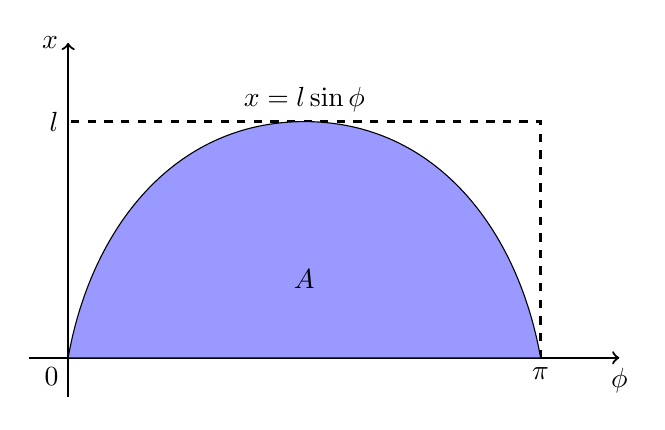
\begin{tikzpicture}
  \draw[->, thick] (-0.5, 0) -- (7, 0)
    node[below] {\(\phi\)};
  \draw[->, thick] (0, -0.5) -- (0, 4)
    node[left] {\(x\)};
  \draw (0, 0) node[below left] {\(0\)};

  \draw (6, 0) node[below] {\(\pi\)};
  \draw (0, 3) node[left] {\(l\)};

  \draw[dashed, thick] (6, 0) -- (6, 3) -- (0, 3);

  \draw[fill = blue!40]
    (0, 0) to[in = 180, out = 80]
    (3, 3) to[in = 100, out = 0]
    (6, 0) -- cycle;
  \draw (3, 1) node {\(A\)};
  \draw (3, 3) node[above] {\(x = l \sin \phi\)};

\end{tikzpicture}